
%===================================
%===================================
\section{Comparaciones}
\label{sec:Comparaciones}

En esta sección se presentan comparaciones entre los diferentes algoritmos implementados, incluyendo el algoritmo secuencial optimizado por compilador, el algoritmo secuencial optimizado por cache line, el algoritmo paralelizado con hilos y el algoritmo paralelizado por procesos. Se analizarán los resultados obtenidos en términos de tiempo de ejecución y speedup para cada caso, destacando las diferencias y similitudes entre las distintas implementaciones. Además, se discutirán las posibles razones detrás de los resultados observados y se ofrecerán conclusiones sobre el rendimiento de cada enfoque en función de los datos recopilados durante las pruebas.

\begin{table}[H]
   \centering
   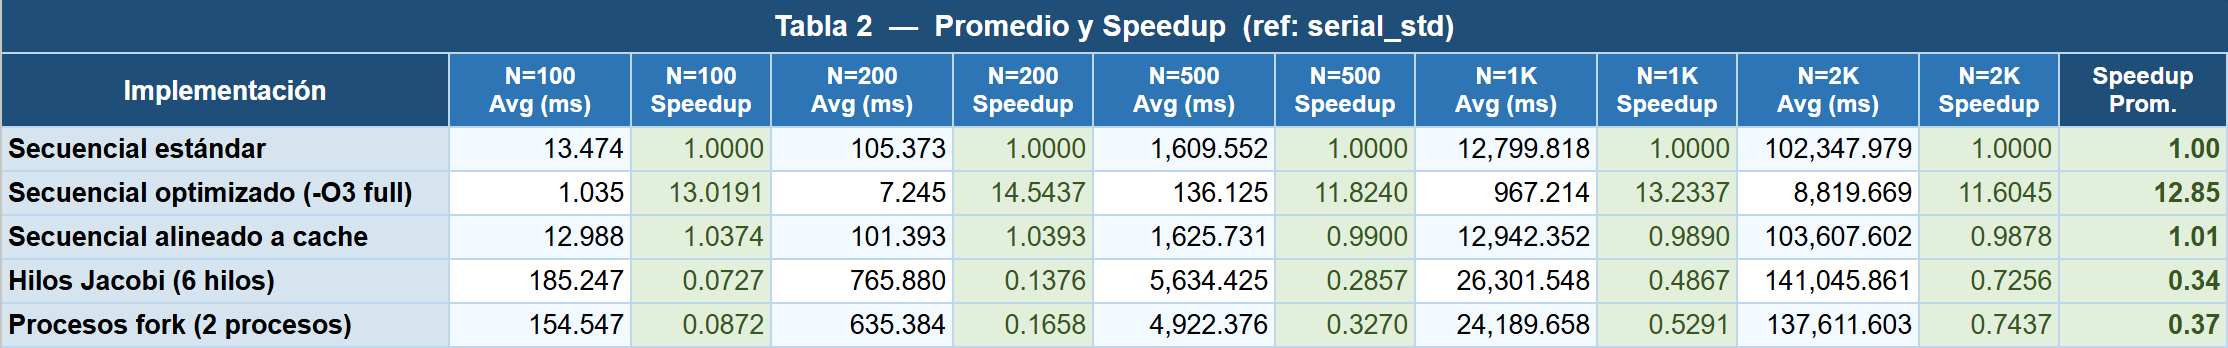
\includegraphics[width=1\textwidth]{images/tables/final_speedup.png}
   \caption{Comparación del speedup entre los diferentes algoritmos} 
\end{table}

\begin{figure}[H]
   \centering
   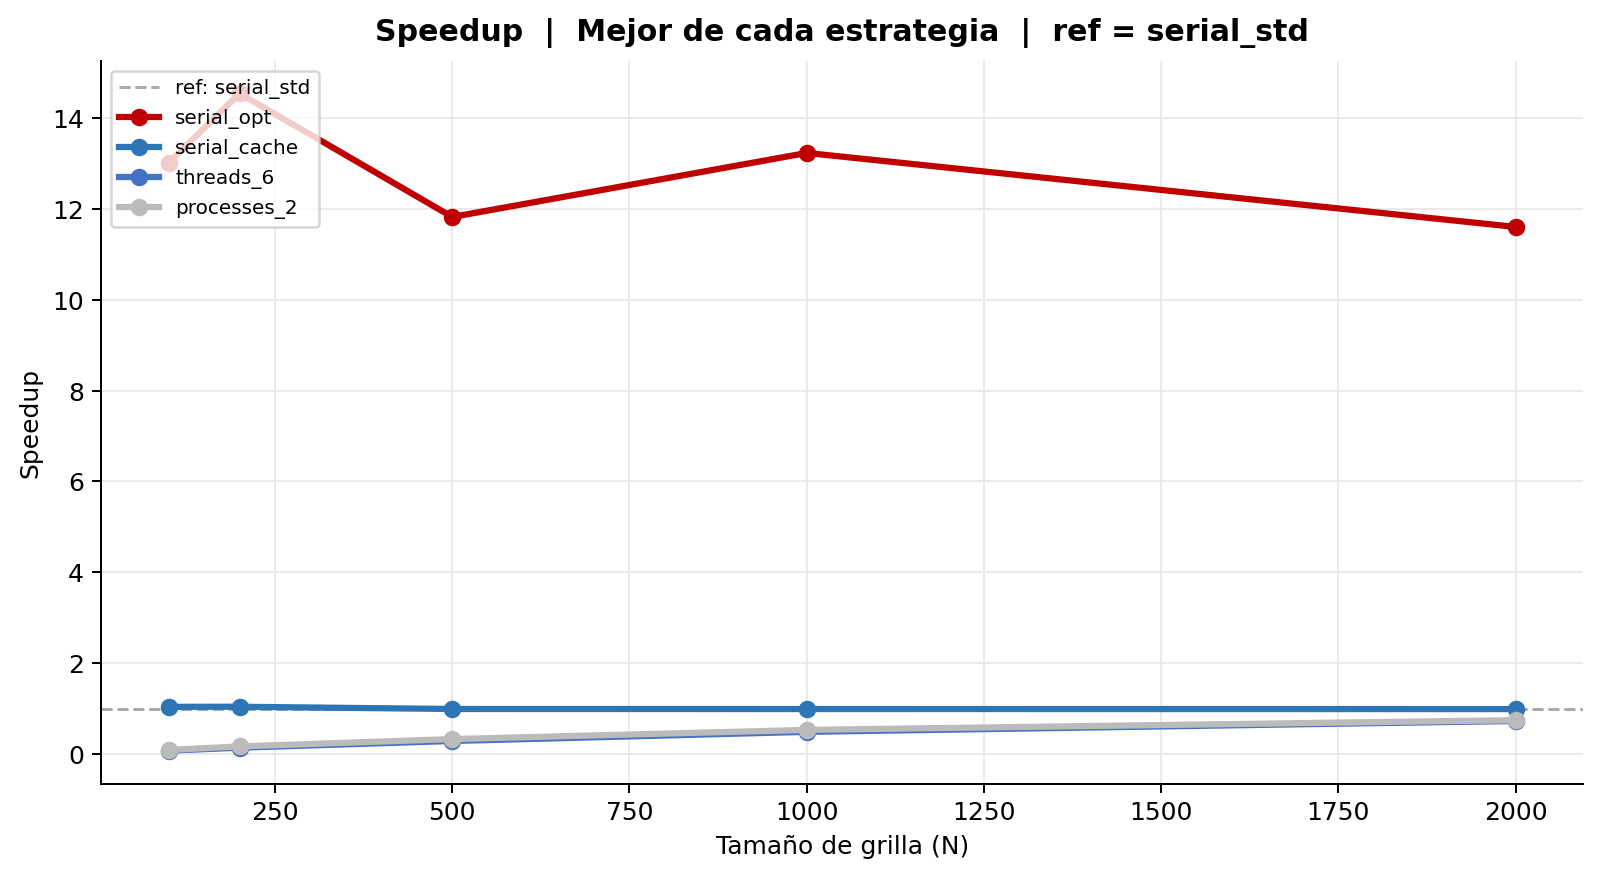
\includegraphics[width=1\textwidth]{images/charts/final_sp.png}
   \caption{Comparación del speedup entre los diferentes algoritmos} 
\end{figure}

\begin{figure}[H]
   \centering
   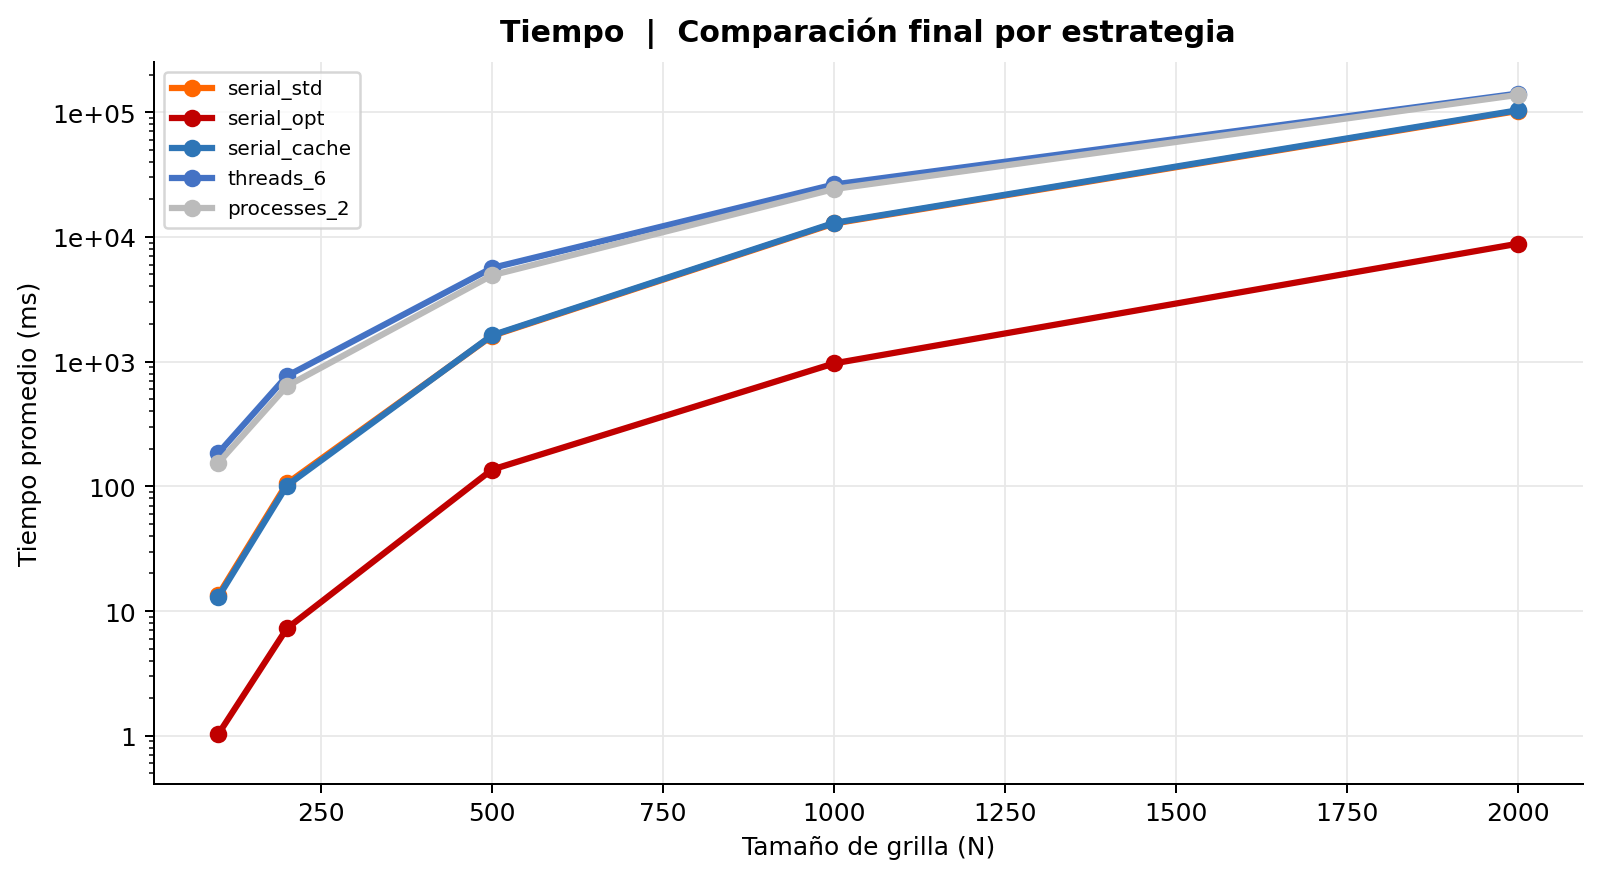
\includegraphics[width=1\textwidth]{images/charts/final_time.png}
   \caption{Comparación del tiempo de ejecución entre los diferentes algoritmos}
   \label{fig:chart_final_time}
\end{figure}


